\chapter{Úvodní sledování}
\begin{wrapfigure}{r}{0.4\textwidth}
    \vspace*{1cm}
    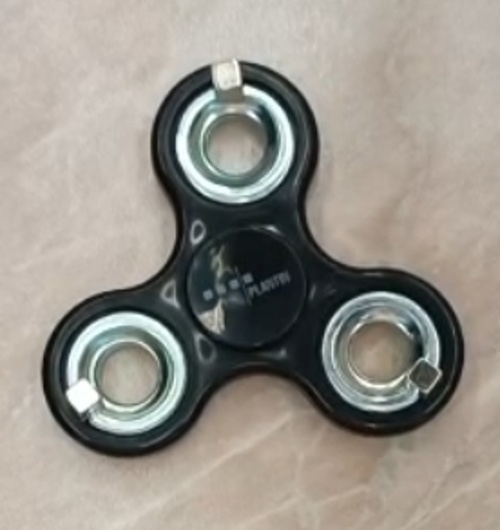
\includegraphics[width=0.3\textwidth]{osazeny_spinner.png}
    \centering
    \caption{Spinner osazený neodymovými magnety}
    \label{fig:1spinner}

    \vspace*{2.5cm}
    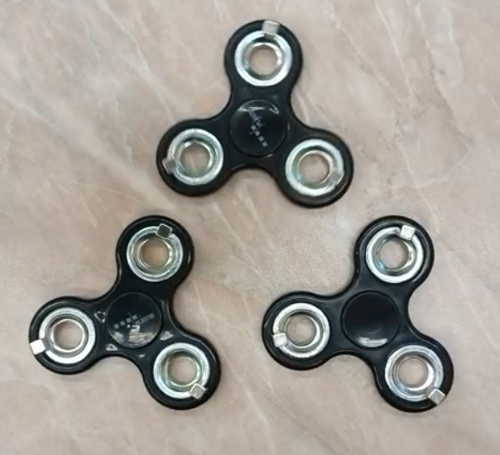
\includegraphics[width=0.35\textwidth]{3spinnery.png}
    \centering
    \caption{Tři interagující spinnery}
    \label{fig:3spinners}
\end{wrapfigure}

Prvním krokem v řešení této úlohy bylo kvalitativní sledování chování spinnerů v několika konfiguracích. Účelem tohoto bylo určení relevantních parametrů a seznámení se s problémem.

Hlavním poznatkem je, že dochází ke změně chování systému dvou spinnerů v závislosti na jejich relativních rychlostech.
Máme-li na stole 2 spinnery, ze kterých je jeden nehybný, a druhý roztočíme na nízkou rychlost, dojde po krátké chvíli k silné a chaotické interakci (záznam experimentu je k vidění v příloze \ref{attachment_1}).
Naopak, roztočíme-li druhý spinner znatelně rychleji, nedochází téměř k žádné interakci (viz příloha \ref{attachment_2}).
Druhý spinner se prvnímu spinneru efektivně jeví jako permanentí magnet - první spinner se tedy nanejvýše umístí do energeticky nejvýhodnější polohy a dále zůstává nehybný.
Dalším cenným poznatkem je, že při interakci více spinnerů se systém chová chaoticky téměř vždy (viz příloha \ref{attachment_3}).
Toto dělá měření interakcí více jak dvou spinnerů složité a za účelem získání použitelných výsledků omezéme náš výzkum pouze na jeden či dva spinnery.
Po vytvoření fyzikálního modelu pro popsání menšího počtu spinnerů se pokusíme o vývoj simulace, která by dovolila větší počty spinnerů.

Ze zadání můžeme také vyčíst další užitěčná omezení.
O umístění všech spinnerů je řečeno, že mají být v \textit{"(jedné) rovině vedle sebe"}. Dále má docházet k točení pouze \textit{"jedním z nich"} a interakce mezi spinnery mají probíhat pouze na bázi \textit{"vlivů magnetického pole"}.
Neměli bychom opomenout ani skutečnost, že všechny spinnery mají být \textit{"identické"}.
\clearpage

\section{Určení parametrů}

Z úvodního sledování není těžké určit relevantní parametry a vybrat, které z nich je možné s naším vybavením měřit. Vybranými parametry se budeme zabývat v následujících kapitolách.

\subsection{Parametry týkající se konfigurace spinnerů}
\label{sub:param_konf}
Jakožto nejdůležitější bychom určitě označili relativní pozice všech spinnerů, které popíšeme pomocí jejich středů $S_1, S_2,...$ (každý střed je braný jako vektor v rovině spinnerů) a jejich poloměrů $r_1, r_2, ...$.
Dále bude k přesnému určení pozic magnetů nezbytné znát okamžitý úhel rotace každého spinneru. Ty ozačíme $\varphi_1, \varphi_2,...$.
Nakonec k popsání spinneru musíme určit počet ramen (neboli počet připevněných magnetů). Tento počet označíme $n$. V našem případě je roven 3.

Pomocí těchto údajů je triviální vyjádřit pozici $P(i)$ libovolného magnetu jeho indexem $i$ (kde $0 \leq i < n$):

\begin{equation}
    \label{eq:magnet_pos}
    P(i) = S + \biggr(r\cos{\bigg(\varphi + \frac{2\pi i}{n}\bigg)},
    r\sin{\bigg(\varphi+\frac{2\pi i}{n}}\bigg), 0 \bigg)
\end{equation}

\begin{wrapfigure}{r}{0.4\textwidth}
    \vspace*{-0.5cm}
    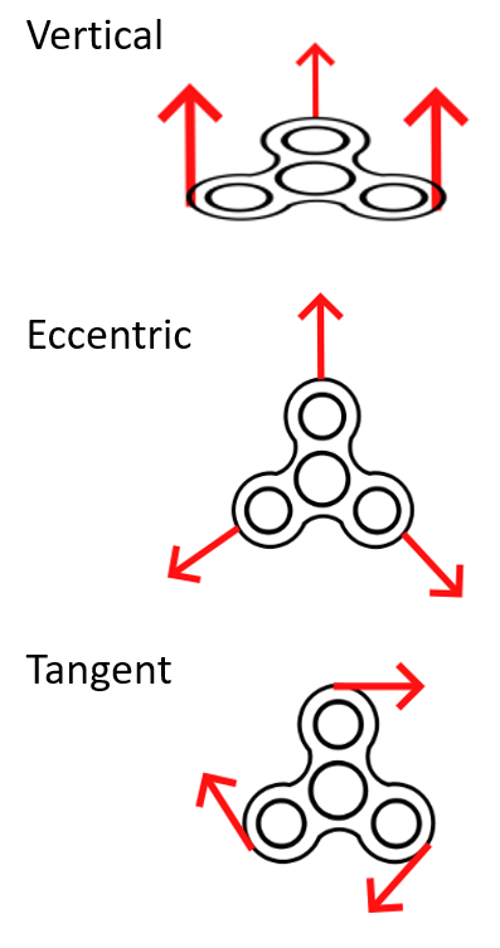
\includegraphics[width=0.3\textwidth]{orientace_magnetu.png}
    \centering
    \caption{Námi vyhrazené orientace magnetů}
    \label{fig:mag_orientations}
\end{wrapfigure}

Kromě pozice magnetu hraje také klíčovou roli nasměrování jeho pólů. Zde definujeme 3 důležité orientace (viz \autoref{fig:mag_orientations}):

\begin{enumerate}[topsep=0pt, partopsep=0pt]
    \setlength{\itemsep}{0pt}%
    \setlength{\parskip}{0pt}%
    \item \textbf{Vertikální (\textit{vertical})}
    \item Odstředivá (\textit{eccentric})
    \item Tečná (\textit{tangent})
\end{enumerate}

V našich experimentech jsme používali převážně vertikální konfiguraci, jelikož takto bylo uchycení magnetů nejjednodušší, protože se magnety samy připevnily ke kovovému závaží umístěnému v každém z ramen spinneru (viz \autoref{fig:1spinner}). Ta jsou zde za účelem zvýšení momentu setrvačnosti spinneru.

Tyto konfigurace jsme také schopni popsat, a to opět jakožto funkci indexu magnetu.
Nejdříve vyjádříme směrový vektor magnetického momentu $\vec{u}(i)$ pro $i$. magnet v každé konfiguraci (viz \autoref{tab:mag_dir_vec})

\vspace{24pt}

\begin{table}[!ht]
    \captionsetup{justification=raggedright,singlelinecheck=off}
    \caption{Směrové vektory pro různé konfigurace}
    \label{tab:mag_dir_vec}

    \def\arraystretch{1.5}
    \begin{tabularx}{\textwidth}{p{0.50\textwidth} p{0.50\textwidth} }
        \textbf{Konfigurace} & \textbf{Směrový vektor magnetu}                    \\
        \hline
        Vertikální           & $\vec{u}(i) = (0,0,1)$                             \\
        Odstředivá           & $\vec{u}(i) = \widehat{P(i) - S}$                  \\
        Tečná                & $\vec{u}(i) = (0,0,1) \times \widehat{(P(i) - S)}$ \\
    \end{tabularx}
\end{table}

{\raggedright
Když nyní zvolíme velikost magnetického momentu našich magnetů $|\vec{m}_0|$, jsme schopni popsat magnetický moment včetně jeho velikosti\footnote{Všimněme si, že $u(i) = \hat{u}(i)$.}:}

\begin{equation}
    \label{eq:magnet_moment_orientation}
    \vec{m} = |\vec{m}_0| \cdot \vec{u}(i)
\end{equation}

Velikost magnetických momentů bude záviset na teplotě, velikosti a materiálových vlastnostech magnetů (např. jejich chemickém složení a kvalitě). Ale to, jaká je pravá velikost magnetických momentů našich magnetů, je momentálně nepodstatné a určíme ji později (viz \autoref{sec:remanence_measurement}).

Posledním parametrem, který zmíníme v této části je, zda se magnety přitahují, či odpuzují.
V našem případě jsme se zaměřili na systémy, kde se všechny magnety odpuzují.

\subsection{Parametry týkající se pohybu spinnerů}
\label{sub:param_move}

Druhou, složitější, částí popisu našeho systému je jeho pohyb a chování v čase.
Zde se nevyhneme úhlovým rychlostem jednotlivých spinnerů, které budeme značit $\omega_1, \omega_2,...$.
Poté nás přirozeně zajímají i jejich úhlová zrychlení $\alpha_1, \alpha_2, ...$. Pro naše výpočty bude také často potřeba využít definice momentu síly a proto ji zmíníme. Definující závislost je následující: $\tau = I\alpha$ (kde $\tau$ značí moment síly a $I$ značí moment setrvačnosti\footnote{Někdy také značeno $J$.} spinneru).
Určení momentu setrvačnosti bude věnována vlastní kapitola (viz \autoref{sec:moment_of_inertia}).

Posledním dynamickým parametrem, který zmíníme, je tření v ložiscích spinnerů a jiné odporové síly působící na spinner.
Těm se budeme do hloubky věnovat v kapitole \ref{chap:drag}.

\clearpage

\section{Modelování magnetů}
V průběhu našich experimentů používáme neodymové (NdFeB) magnety krychlového tvaru o hraně 5mm a jakosti N35\footnote{Jakosti neodymových magnetů se pohybují od N35 do N55 \cite{magnet_grades}.}.
Toto standardní označení jakosti neodymových magnetů popisuje jejich chemické složení, tepelnou odolonost a hlavně magnetickou sílu \cite{magnet_grades}, která je popsána pomocí tzv. remanentní magnetizace, neboli remanence.

Jelikož jsou magnety poměrně malé, můžeme je ve větších vzdálenostech aproximovat jakožto magnetické dipóly.
Zároveň existuje velmi elegantní způsob, jak vypočítat velikost magnetického dipólu z jeho remanence \cite{magnetic_torque}:

\begin{equation}
    \label{eq:mag_mom_remanence}
    |\vec{m}_0| = \frac{1}{\mu_0}|\vec{B}_r|V
\end{equation}

Tabulkové hodnoty pro remanenci NdFeB magnetů jsou sice známé, ale v našem případě budeme přesnou hodnotu $|\vec{B}_r|$ našich magnetů měřit později, v kapitole \ref{sec:remanence_measurement}.

\section{Popis magnetických interakcí}

Jelikož k popisu magnetů používáme idealizaci pomocí magnetických dipólů, můžeme popsat interakce mezi nimi pomocí následujících rovnic.
Hlavní interakce mezi dvěma magnetickými dipóly jsou:
\begin{enumerate}[topsep=0pt, partopsep=0pt]
    \setlength{\itemsep}{0pt}%
    \setlength{\parskip}{0pt}%

    \item Silové interakce \cite{magnetic_force} mezi dvěma momenty $\vec{m}_1$ a $\vec{m}_2$, které jsou od sebe vzdáleny\footnote{$\vec{r} = P_1 - P_2$} $\vec{r}$:

          \begin{equation}
              \label{eq:F_m}
              \begin{split}
                  F_m (r,m_1,m_2) = \frac{3\mu_0}{4\pi ||r||^5}
                  \bigg[
                      (m_1\cdot r) m_2 +
                      (m_2\cdot r) m_1 +
                      (m_1\cdot m_2) r -
                      \frac{5(m_1\cdot r)(m_2\cdot r)}{||r||^2} r
                  \bigg] \\
              \end{split}
          \end{equation}

    \item Magnetické interakce, neboli působení momentu síly \cite{magnetic_torque} na $\vec{m}_2$ z důvodu vytvoření magnetického pole $B(r, m_1)$ momentem $\vec{m}_1$ \cite{magnetic_force}:

          \begin{equation}
              \label{eq:B}
              \begin{split}
                  B (r, m) = \frac{\mu_0}{4\pi}\frac{3 \hat{r}(\hat{r}\cdot m) - m}{|r|^3} \\
                  \tau = m_2 \times B(r, m_1)
              \end{split}
          \end{equation}
\end{enumerate}
